% \documentclass[bwprint]{cumcmthesis} %去掉封面与编号页
\documentclass[withoutpreface,bwprint]{cumcmthesis} %去掉封面与编号页
\newcommand{\diff}{\mathop{}\!\mathrm{d}} % 正体微分符号

\usepackage{graphicx}       % 用于插入图片
\usepackage{subcaption} 
\usepackage{algorithm}
\usepackage{algorithmic} % 导言区需添加这两个宏包
\usepackage{comment}  

\usepackage{booktabs}
\usepackage{tabularx}
\usepackage{float}
\usepackage[numbers]{natbib}

\title{基于统计学习方法的NIPT时点选择与胎儿的异常判定决策模型}
\tihao{C}
\baominghao{1234}
\schoolname{中原工学院}
\membera{杨帅博}
\memberb{洪宜昕}
\memberc{宋诗昊}
\supervisor{魏冰蔗}
\yearinput{2025}
\monthinput{09}
\dayinput{07}


\begin{document}

% 标题
\maketitle
\nocite{*}
\bibliographystyle{gbt7714-numerical}

\begin{abstract}

    \textbf{针对问题一,}

    \textbf{针对问题二,}

    \textbf{针对问题三,}

    \textbf{针对问题四,}

    \keywords{}
\end{abstract}

% 问题背景与重述
\section{问题重述}
NIPT(Non-invasive Prenatal Test,即无创产前检测)是一种通过采集母体血液、检测胎儿的游离DNA 片段、分析胎儿染色体是否存在异常的产前检测技术,目的是通过早期检测确定胎儿的健康状况。根据临床经验,畸型胎儿主要有唐氏综合征、爱德华氏综合征和帕陶氏综合征,这三种体征分别由胎儿21 号、18 号和 13 号“染色体游离 DNA 片段的比例”(简称“染色体浓度”)是否异常决定。NIPT 的准确性主要由胎儿性染色体(男胎 XY,女胎 XX)浓度判断。通常孕妇的孕期在 10 周~25 周之间可以检测胎儿性染色体浓度,且如果男胎的 Y 染色体浓度达到或高于 4%、女胎的 X 染色体浓度没有异常,则可认为 NIPT 的结果是基本准确的,否则难以保证结果准确性要求。同时,实际中应尽早发现不健康的胎儿,否则会带来治疗窗口期缩短的风险,早期发现(12 周以内)风险较低;中期发现(13-27 周)
风险高;晚期发现(28 周以后)风险极高。实践表明,男胎 Y 染色体浓度与孕妇孕周数及其身体质量指数(BMI)紧密相关。通常根据孕妇的
BMI 值进行分组(例如:[20,28),[28,32),[32,36),[36,40),40 以上)分别确定 NIPT 的时点(相对孕期的时间点)。由于每个孕妇的年龄、BMI、孕情等存在个体差异,对所有孕妇采用简单的经验分组和统一的检测时点进行 NIPT,会对其准确性产生较大影响。因此,依据 BMI 对孕妇进行合理分组,确定各不同群组的最佳 NIPT 时点,可以减少某些孕妇因胎儿不健康而缩短治疗窗口期所带来的潜在风险。为了研究各类孕妇群体合适的 NIPT 时点,并对检测的准确性进行分析,附件给出了某地区(大多为高 BMI)孕妇的 NIPT 数据。在实际检测中,经常会出现测序失败(比如:检测时点过早和不确定因素影响等)的情况。同时为了增加检测结果的可靠性,对某些孕妇有多次采血多次检测或一次采血多次检测的情况。试利用附件提供的数据建立数学模型研究如下问题:

\textbf{问题1:}
分析胎儿 Y 染色体浓度与孕妇的孕周数和 BMI 等指标的相关特性,给出相应的关系模型,并检验其显著性。

\textbf{问题2:}
男胎孕妇的 BMI 是影响胎儿 Y 染色体浓度的最早达标时间的主要因素。要求对男胎孕妇的 BMI 进行合理分组,给出每组的 BMI 区间和最佳 NIPT时点,使得孕妇可能的潜在风险最小,并分析检测误差对结果的影响。

\textbf{问题3:}

\textbf{问题4:}

% 问题分析
\section{问题分析}

\subsection{问题一分析}

\subsection{问题二分析}


男胎 Y 染色体浓度达标时间受多种因素(身高、体重、年龄等)的影响,试综合考虑这些因素、检测误差和胎儿的 Y 染色体浓度达标比例(即浓度达到或超过 4\%的比例),根据男胎孕妇的 BMI,给出合理分组以及每组的最佳 NIPT 时点,使得孕妇潜在风险最小,并分析检测误差对结果的影响。

问题 4 由于孕妇和女胎都不携带 Y 染色体,重要的是如何判定女胎是否异常。试以女胎孕妇的 21
号、18 号和 13 号染色体非整倍体(AB 列)为判定结果,综合考虑 X 染色体及上述染色体的 Z 值、GC
含量、读段数及相关比例、BMI 等因素,给出女胎异常的判定方法。



% 问题分析
\section{问题分析}


% 模型假设
\section{模型假设}




% 符号说明
\section{符号说明}


% 模型建立与求解
\section{模型建立与求解}

\subsection{问题一模型的建立与求解}
\subsubsection{数据预处理}
判断空数据,异常数据除去

首先认为存在相关性,叙述相关性,代入数据算出相关性,根据结果描述相关性强弱。

相关系数 皮尔逊 斯庇尔曼 肯德尔相关系数 效果皮尔逊最好 

p检验t检验

散点图 热力图

低于0.05显著性比较强

\begin{figure}[H]
    \centering
    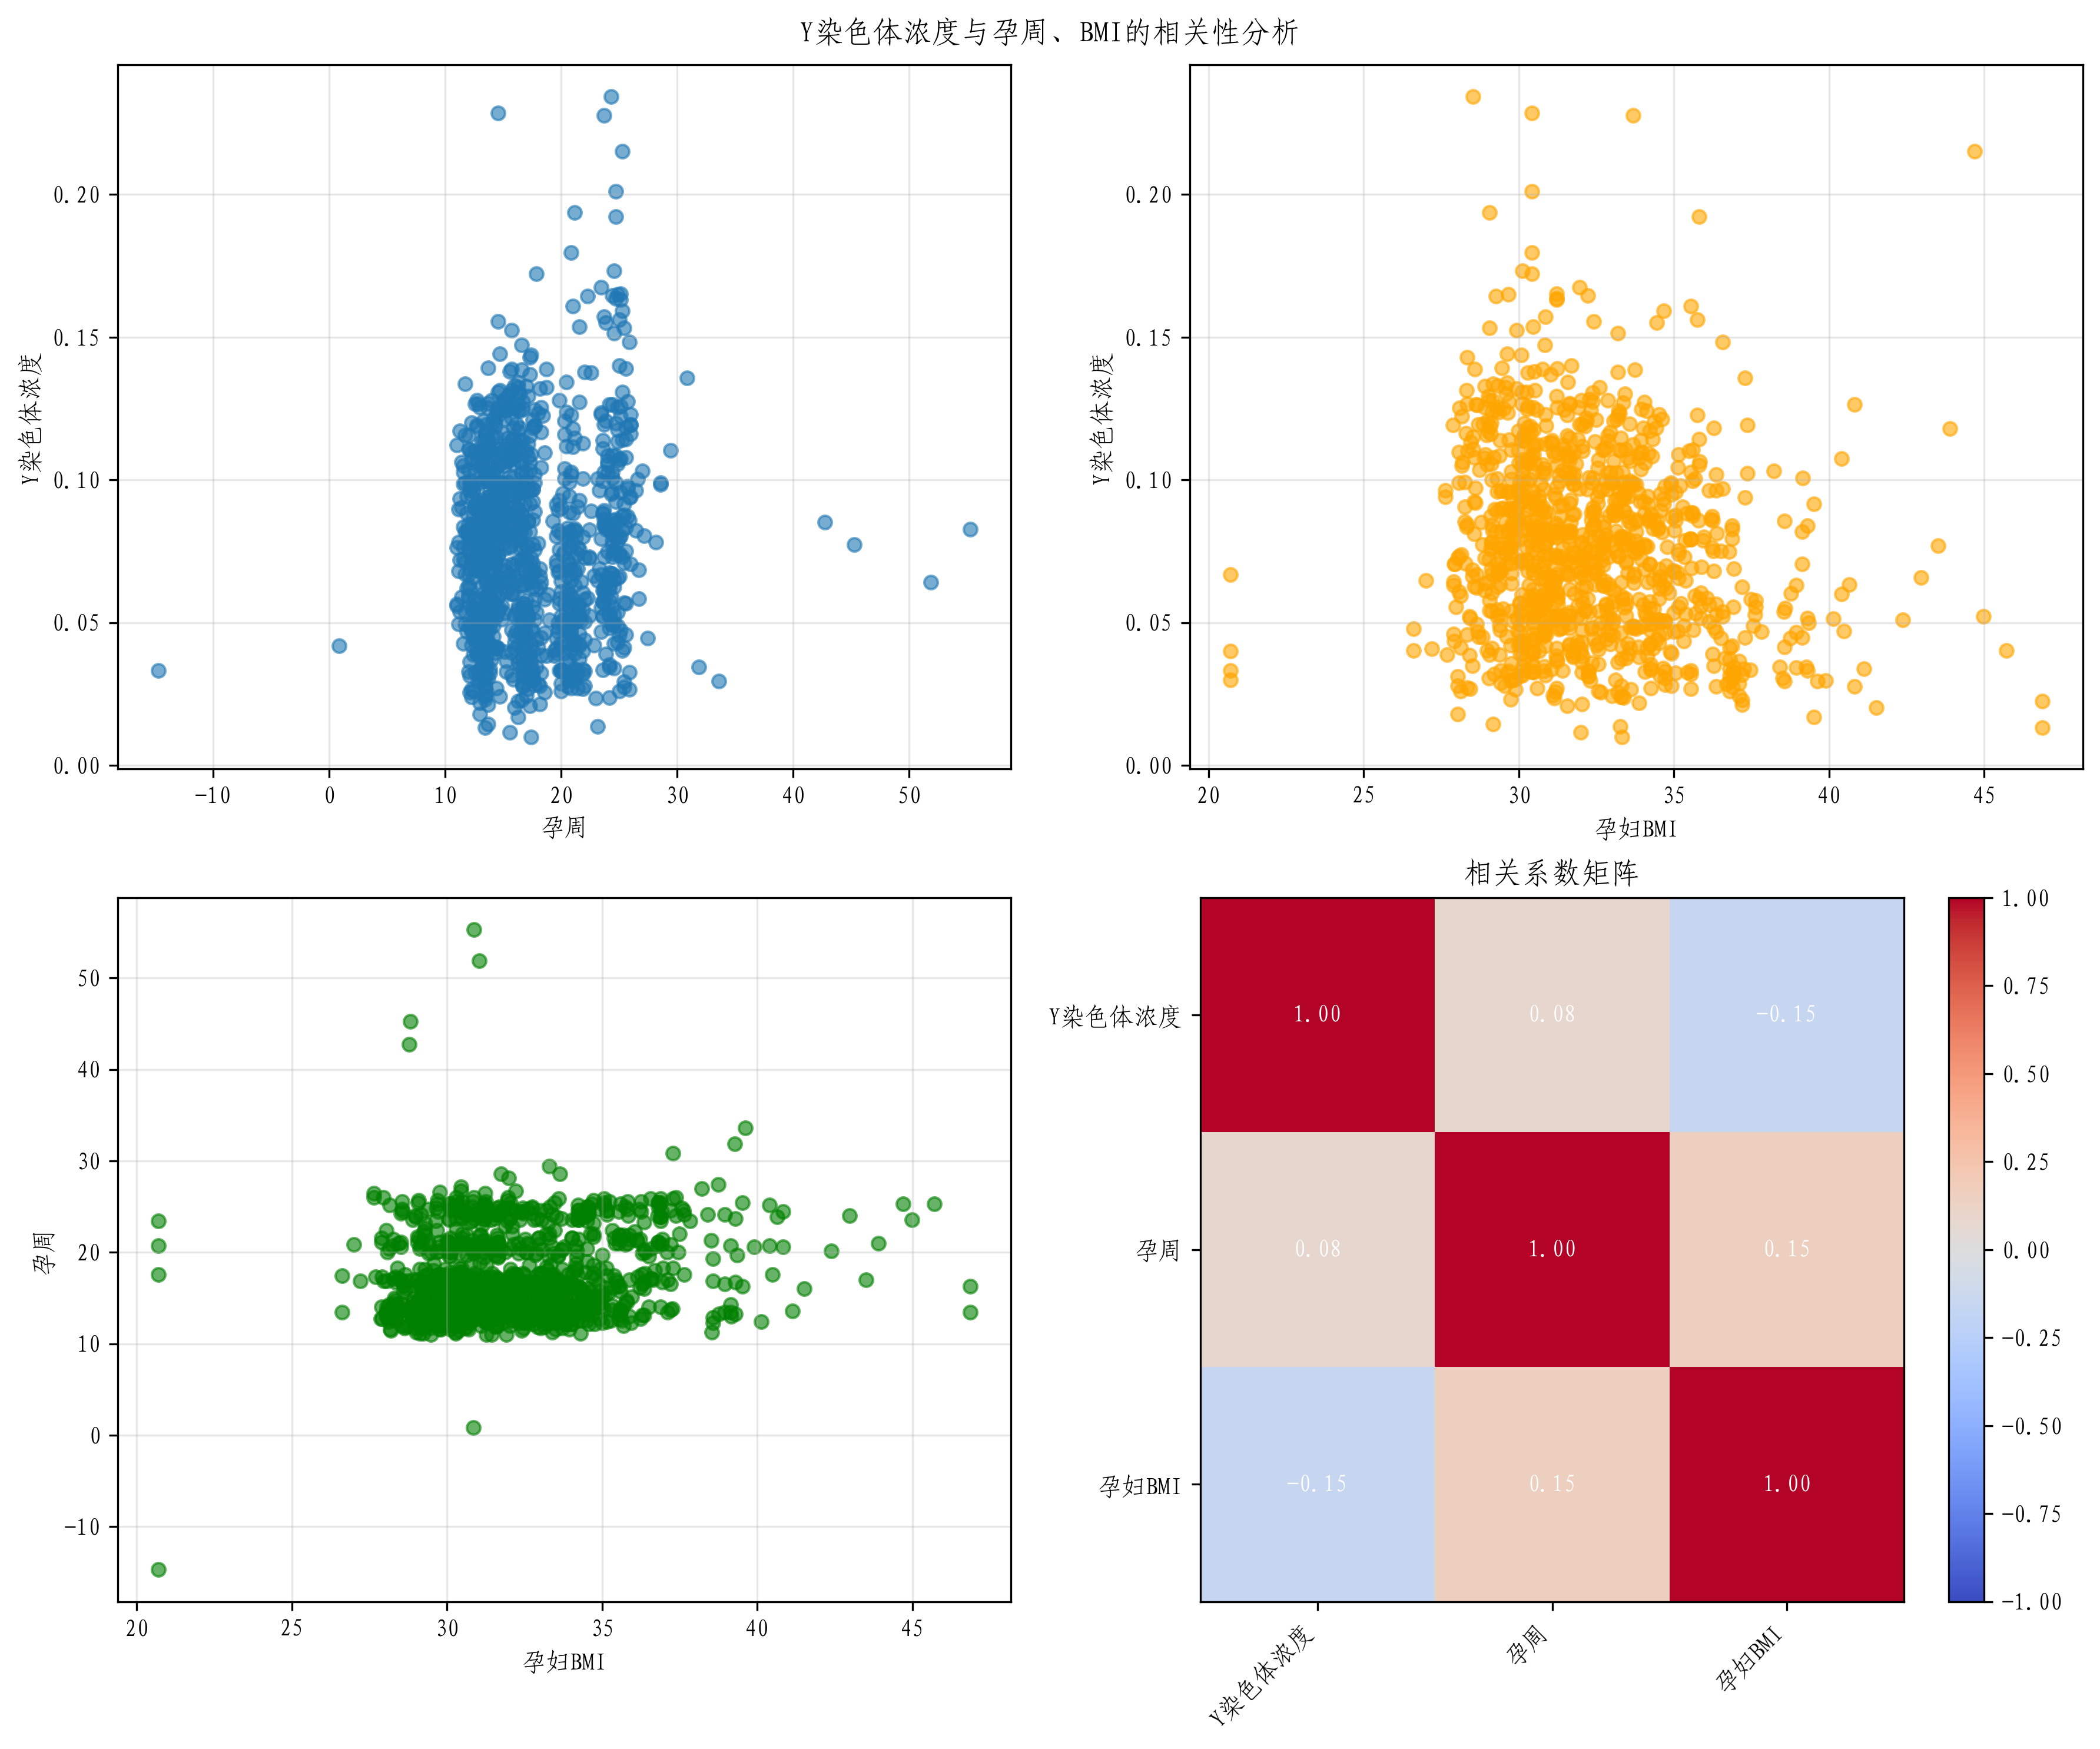
\includegraphics[width=0.8\textwidth]{../figure/q1_1.png}
    \caption{Y染色体密度与孕周、BMI散点图}
    \label{fig:heatmap}
\end{figure}

\begin{figure}[H]
    \centering
    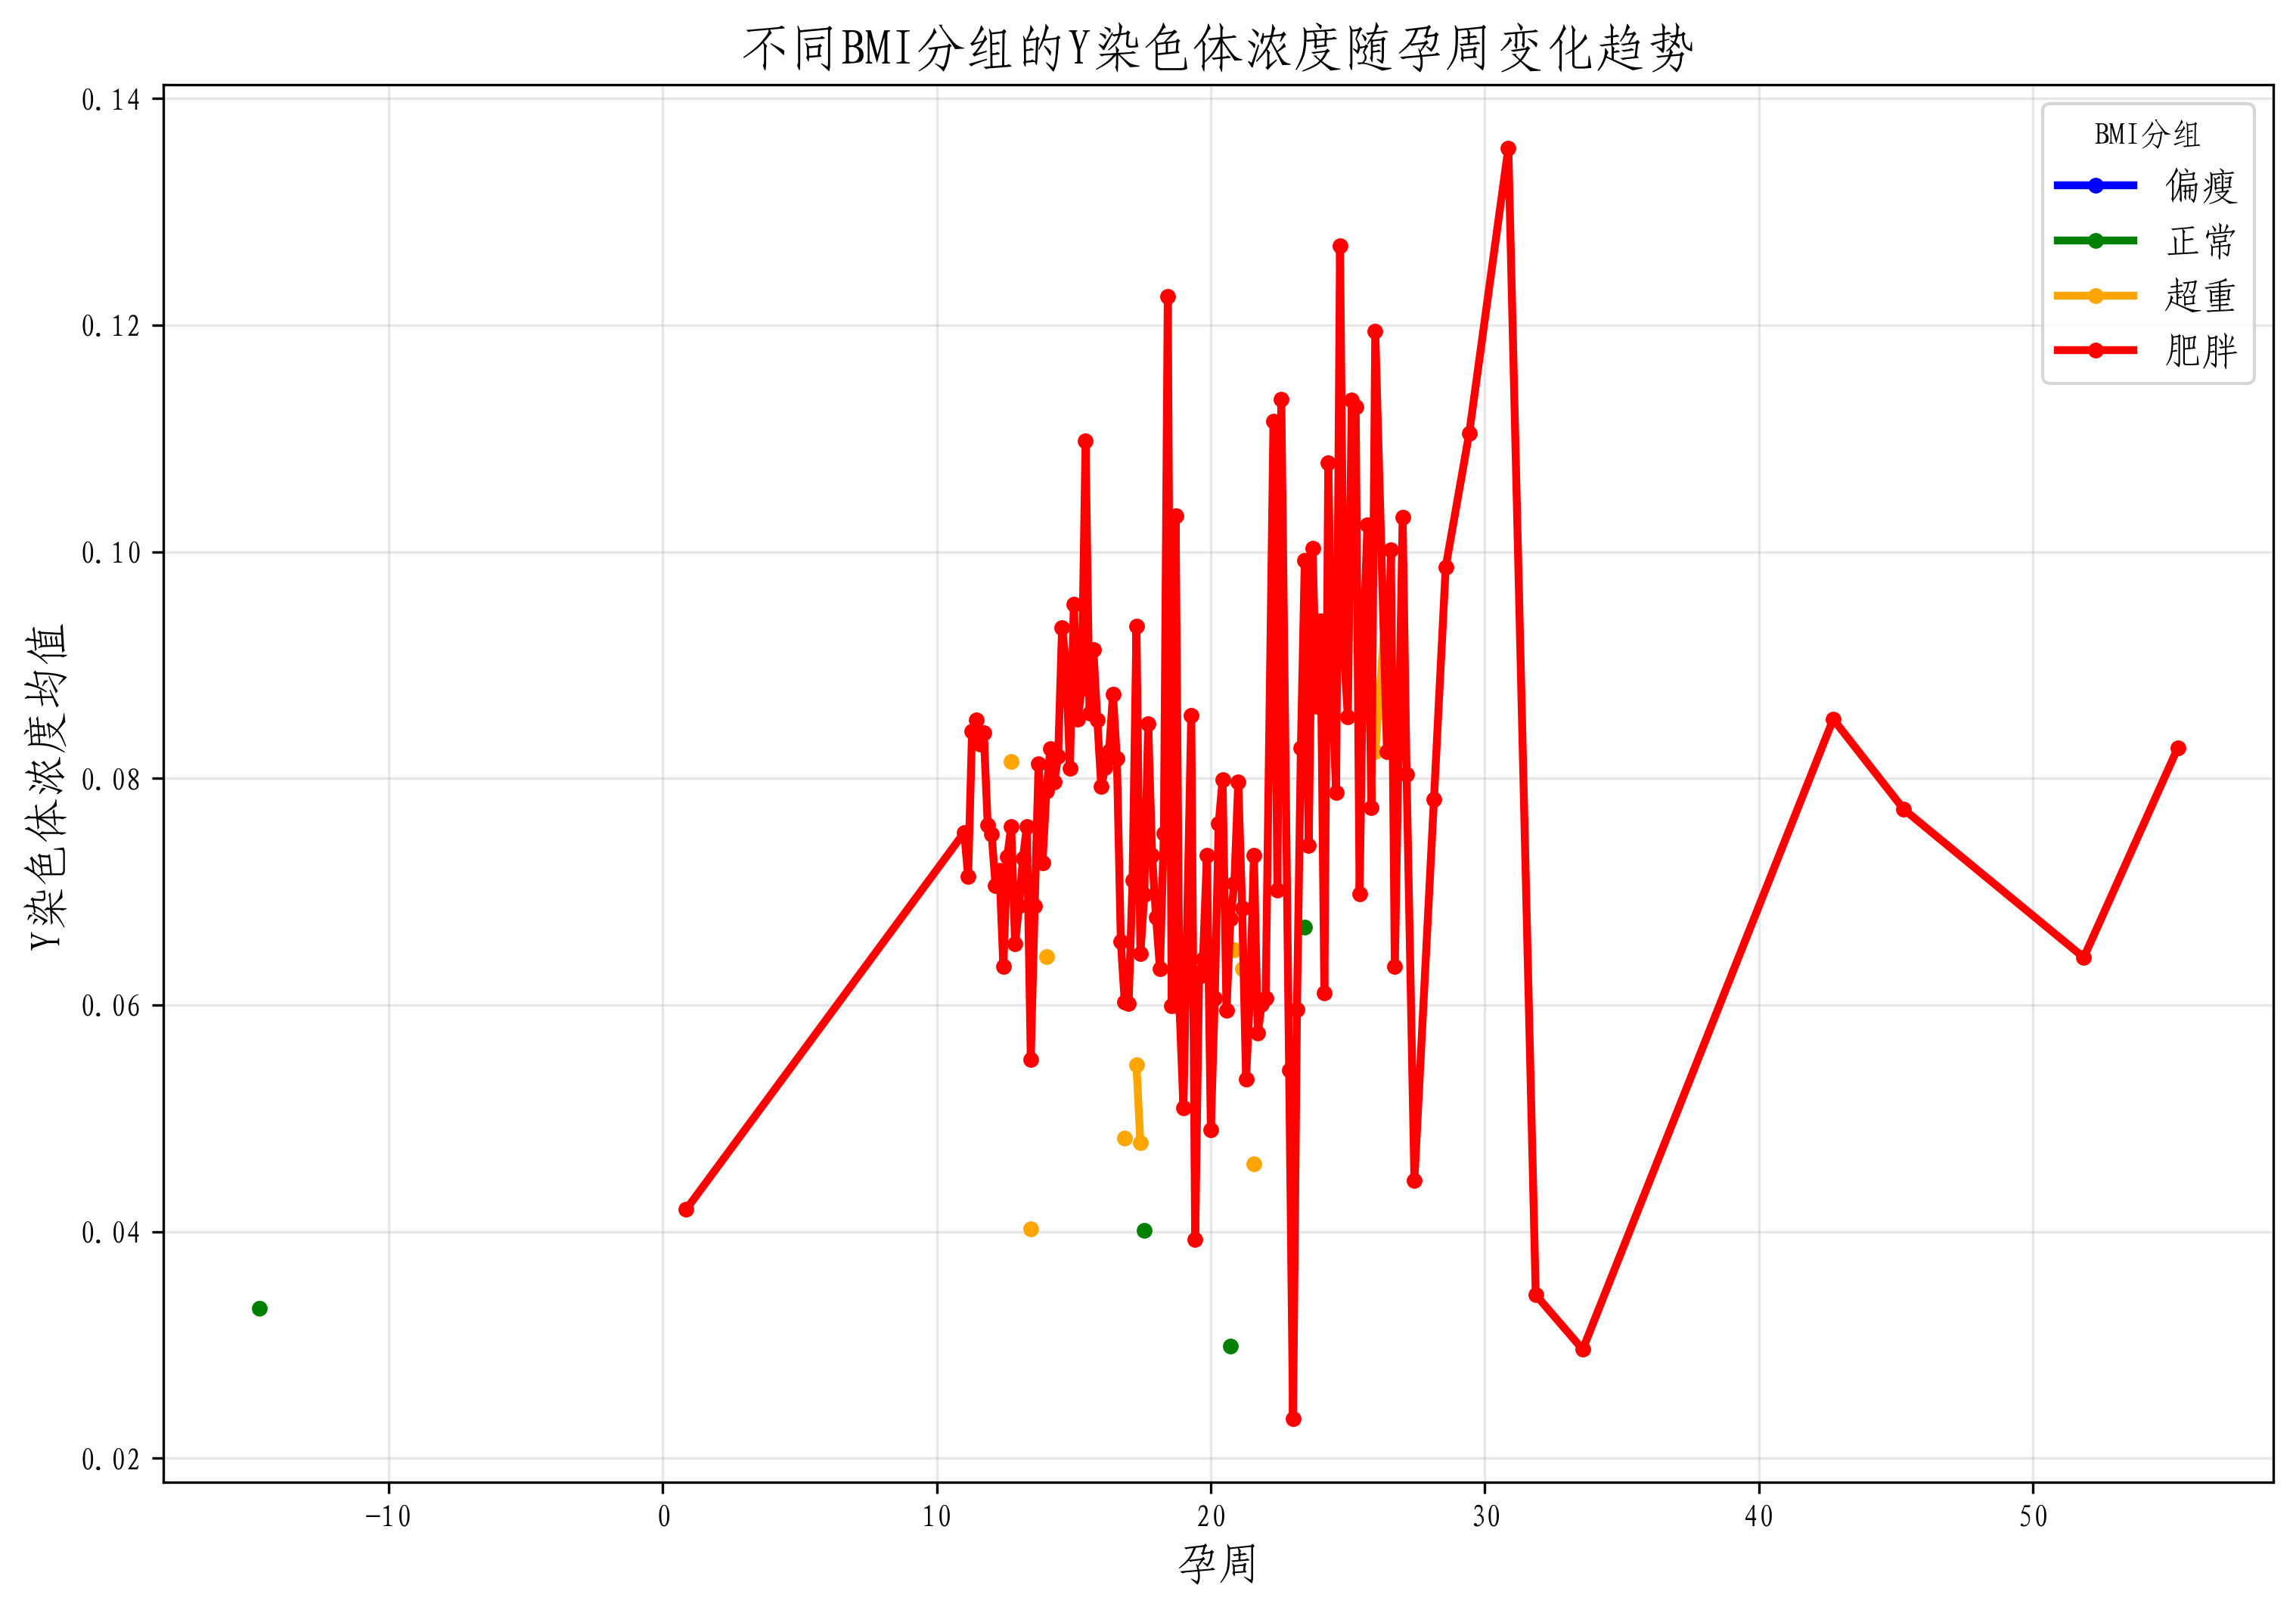
\includegraphics[width=0.8\textwidth]{../figure/q1_2.png}
    \caption{不同BMI分组的Y染色体浓度随孕周变化趋势图}
    \label{fig:heatmap}
\end{figure}

\begin{figure}[H]
    \centering
    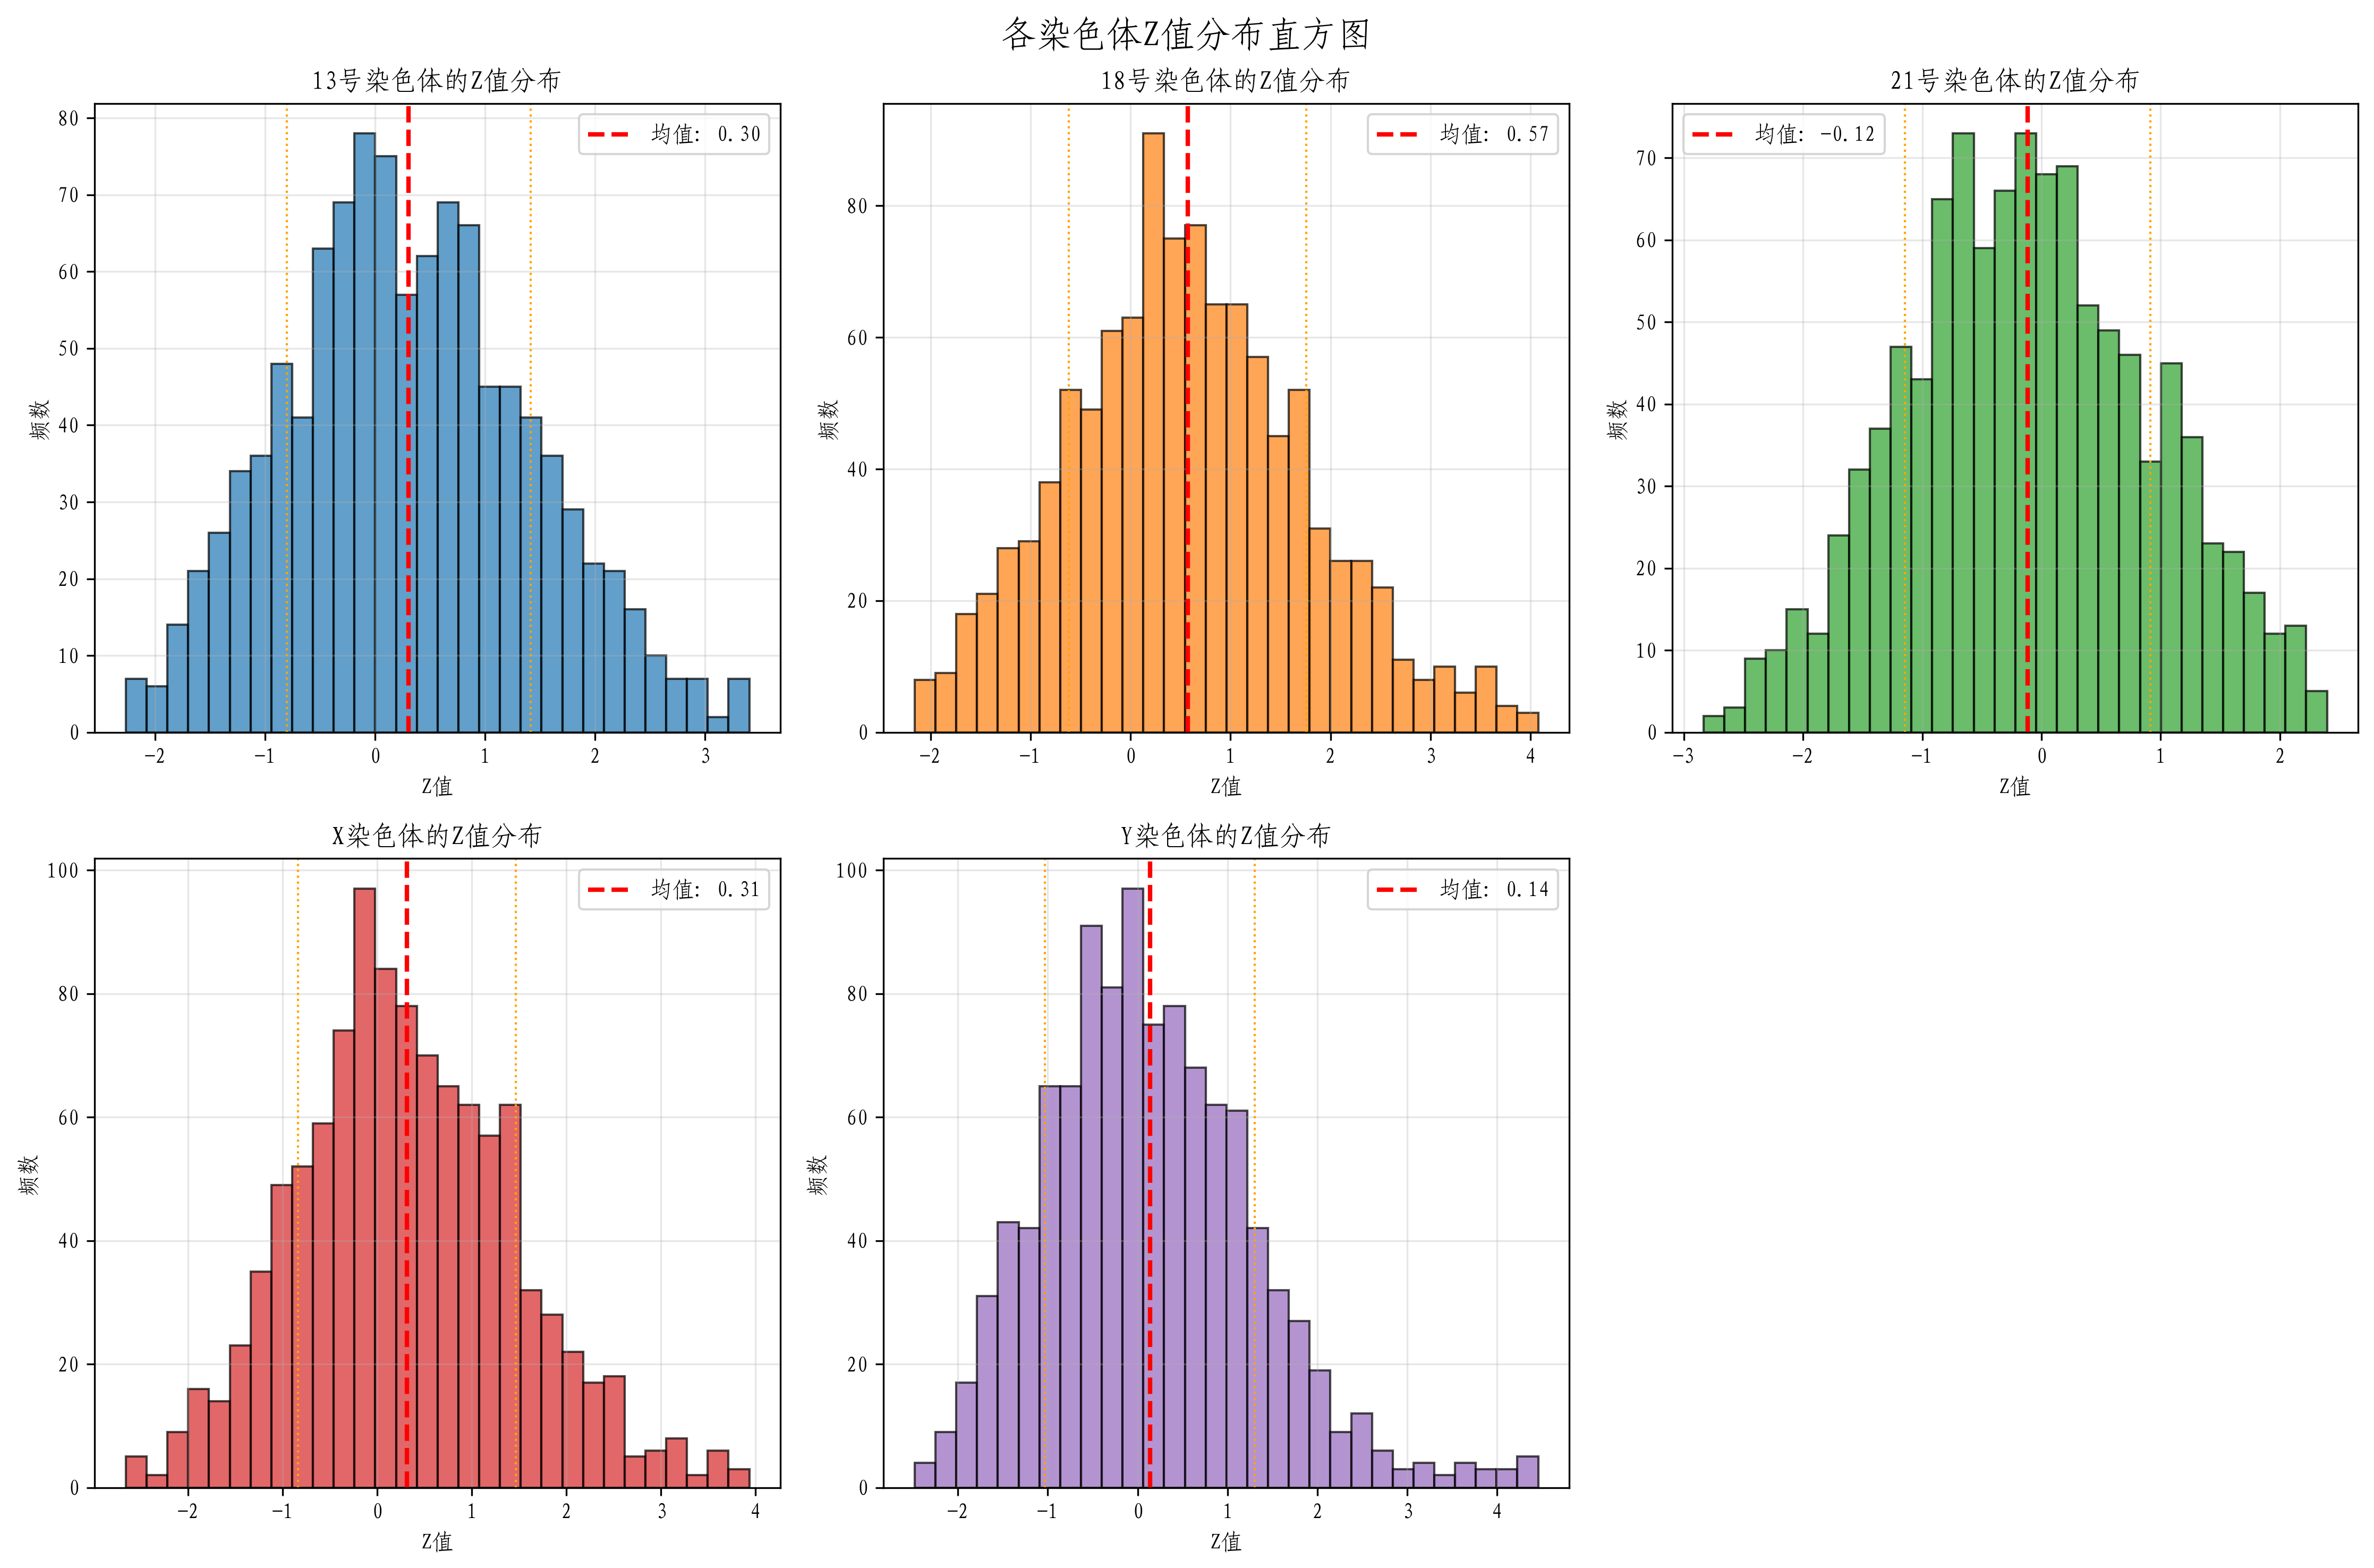
\includegraphics[width=0.8\textwidth]{../figure/q1_3.png}
    \caption{各染色体Z值的分布直方图}
    \label{fig:heatmap}
\end{figure}

\begin{figure}[H]
    \centering
    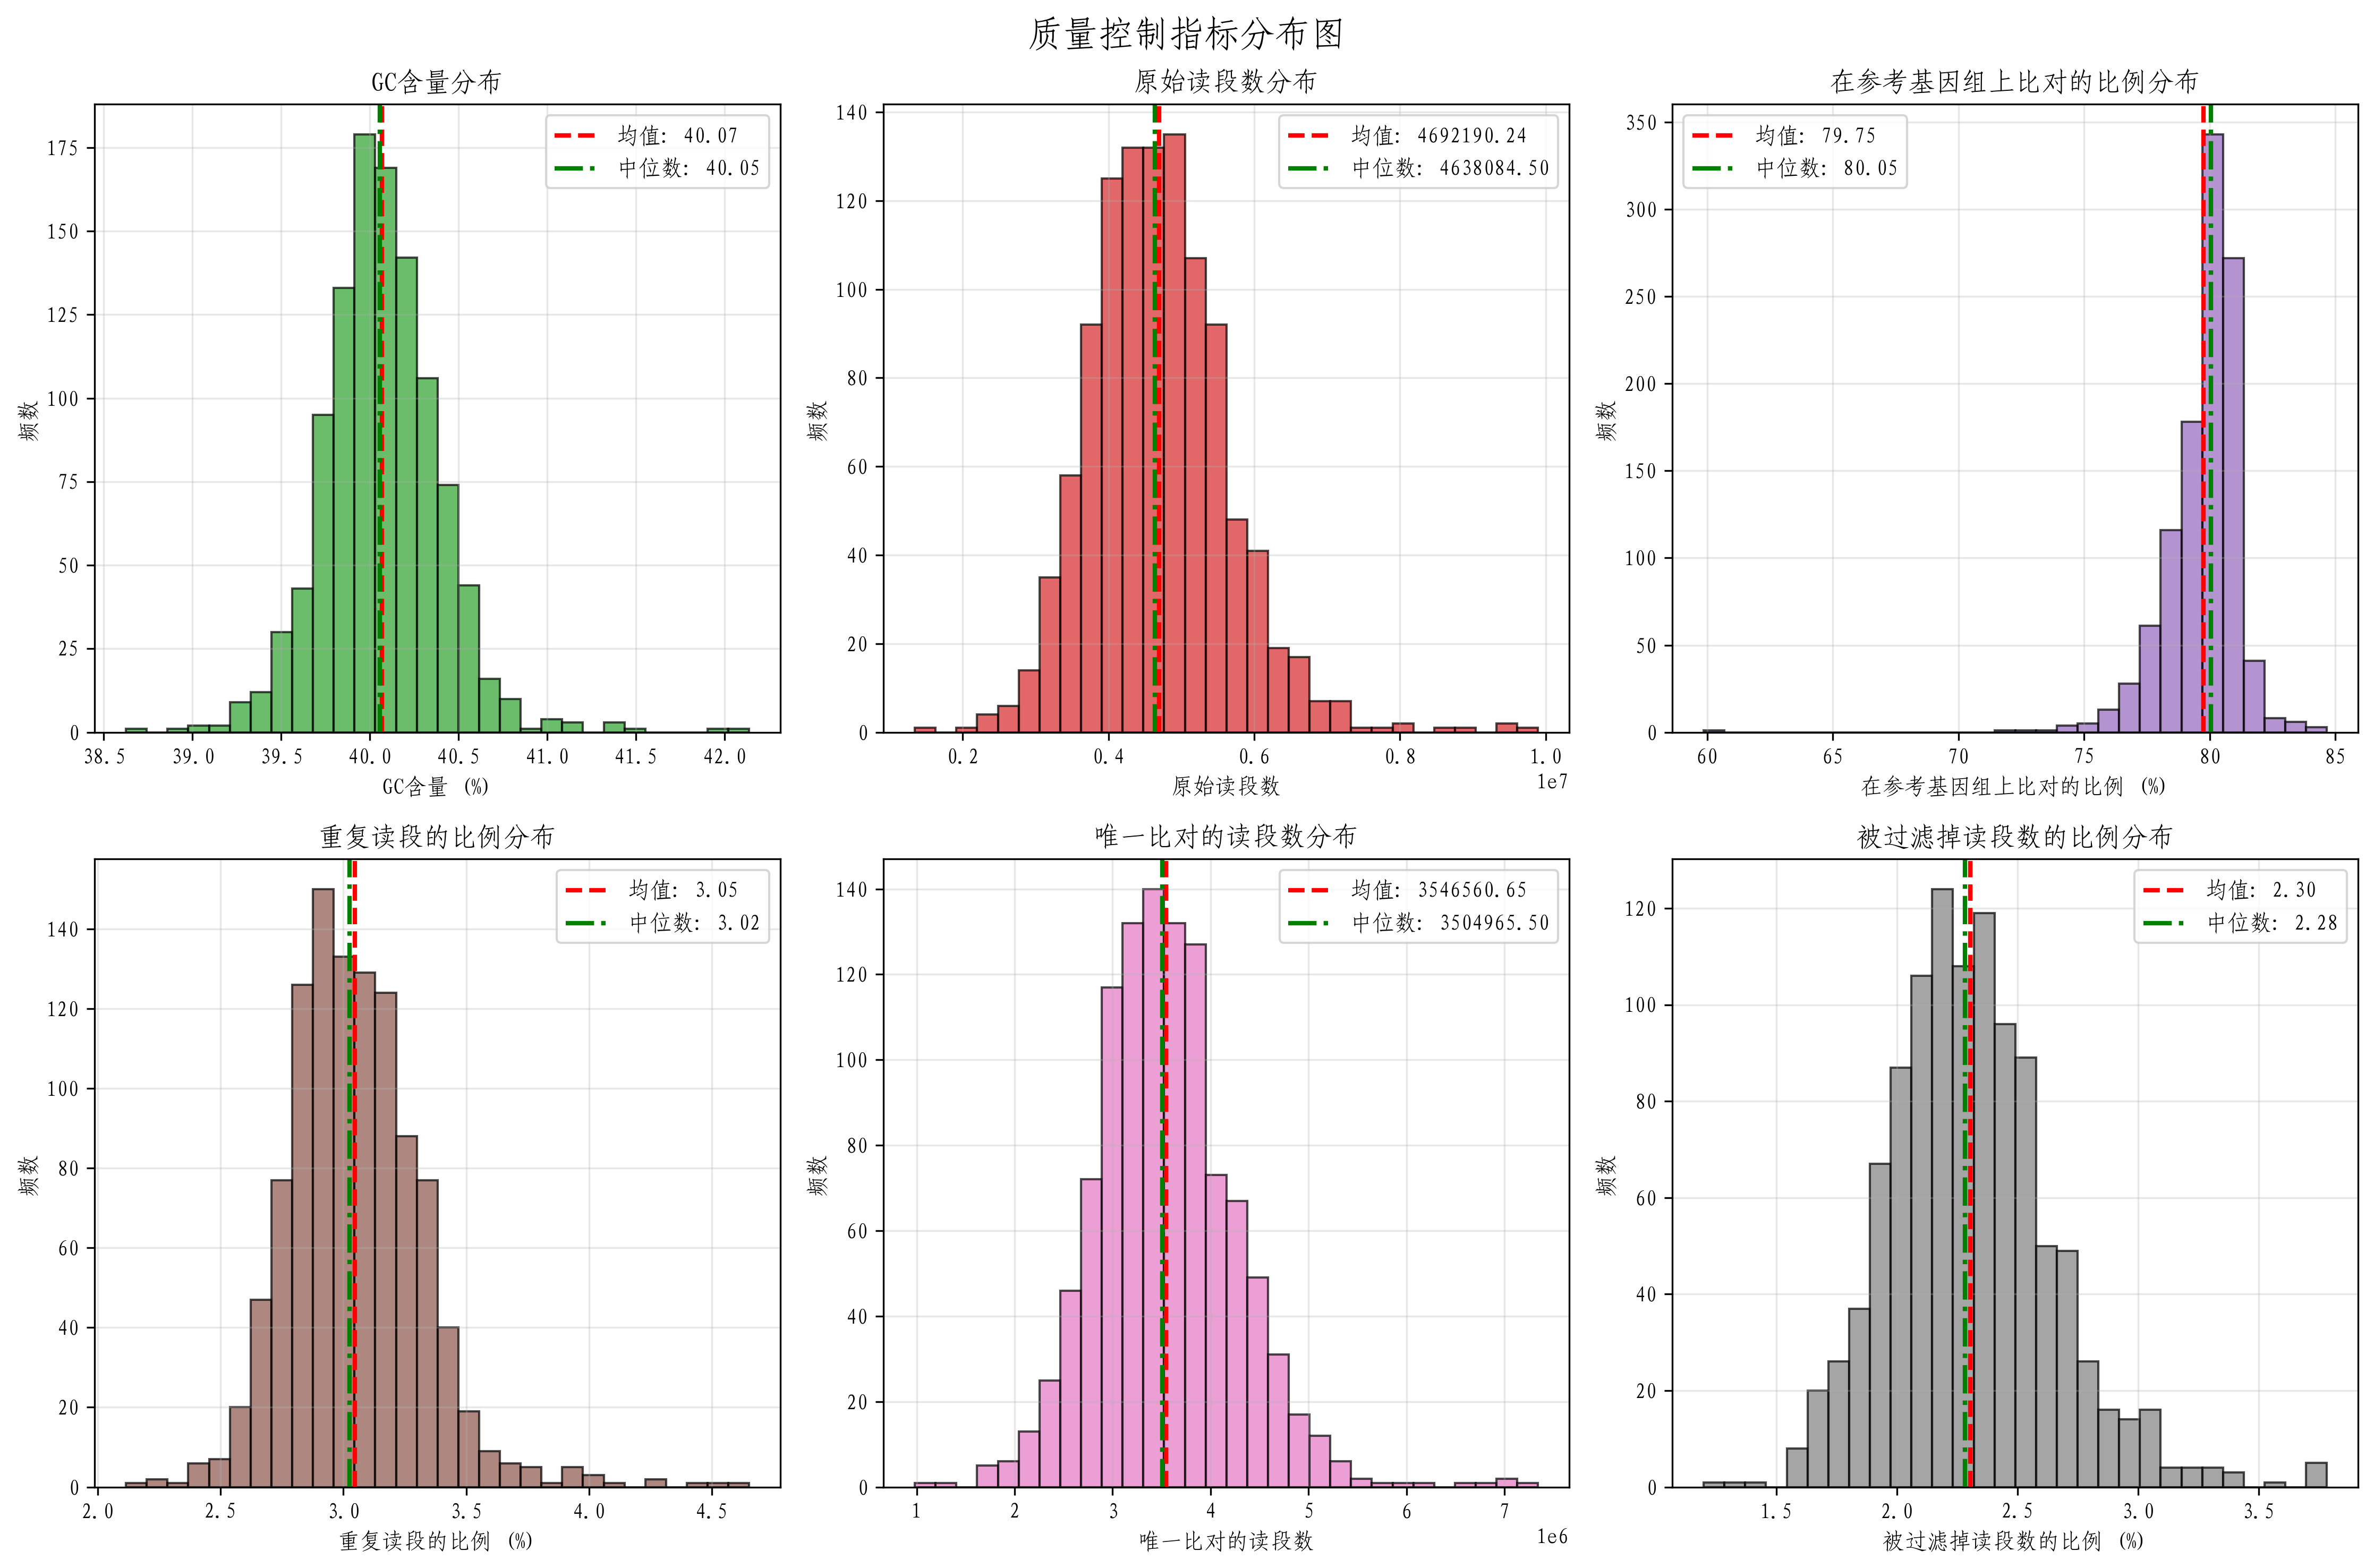
\includegraphics[width=0.8\textwidth]{../figure/q1_4.png}
    \caption{质量控制指标分布图}
    \label{fig:heatmap}
\end{figure}





\subsection{问题二模型的建立与求解}

\subsection{问题三模型的建立与求解}

\subsection{问题四模型的建立与求解}

% 模型评价
\section{模型评价}
\subsection{模型优点}

\subsection{模型缺点}

% 摘要
\bibliography{ref}

% 附录

\begin{appendices}
    % \section{附录名}
\end{appendices}

\end{document}